\documentclass{article}
\usepackage[margin=1in]{geometry}
\usepackage{amsmath}
\usepackage{amssymb}
\usepackage{enumitem}
\usepackage{tikz}

% Tree notation: state on the left, branches labelled H / T,
% leaf = contribution (cost of toss + expectation from new state) x probability.
\tikzset{
  tr/.style={font=\normalsize},
  br/.style={thick},
  lb/.style={midway, above, sloped, font=\small}
}

\begin{document}

\section*{First-Step Analysis: Interview Questions and Answers}

\subsection*{How to read the trees}

$E_s$ is the expected number of \emph{additional} tosses from state $s$.
Each branch is one toss. A leaf shows
\[
(\text{new state's expectation} + 1)\times(\text{probability of that branch}),
\]
where the $+1$ pays for the toss just made. A leaf that stops the game shows $1\times$ probability.
Adding the leaves gives the equation for the state.

\subsection*{Question 0: Expected Tosses Until HH}

\textbf{Question:}
A fair coin is tossed until two Heads appear in a row (HH). What is the expected number of tosses?

\begin{center}
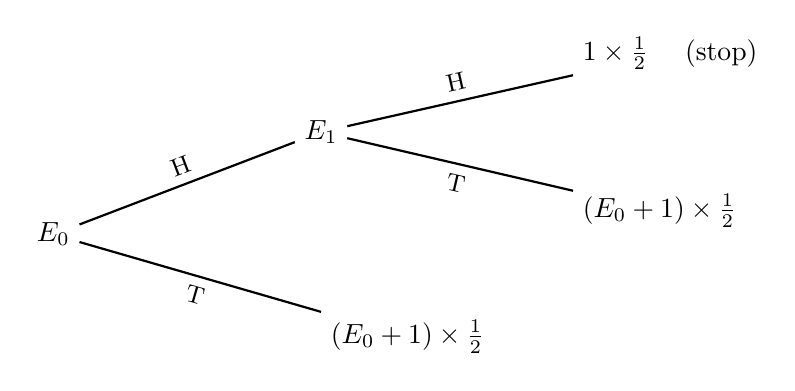
\begin{tikzpicture}[tr]
  \node (e0) at (0,0) {$E_0$};
  \node (e1) at (3.4,1.3) {$E_1$};
  \node[anchor=west] (t0) at (3.4,-1.3) {$(E_0+1)\times\tfrac12$};
  \node[anchor=west] (h1) at (6.6,2.3) {$1\times\tfrac12$ \quad (stop)};
  \node[anchor=west] (t1) at (6.6,0.3) {$(E_0+1)\times\tfrac12$};
  \draw[br] (e0) -- node[lb]{H} (e1);
  \draw[br] (e0) -- node[lb,below]{T} (t0);
  \draw[br] (e1) -- node[lb]{H} (h1);
  \draw[br] (e1) -- node[lb,below]{T} (t1);
\end{tikzpicture}
\end{center}

\textbf{Answer:}

Reading the leaves of the tree:

\[
E_1=\tfrac12(1)+\tfrac12(E_0+1)=1+\tfrac12E_0 \quad\text{(1)}
\]
\[
E_0=\tfrac12(E_1+1)+\tfrac12(E_0+1)=\tfrac12E_1+\tfrac12E_0+1 \quad\text{(2)}
\]

Put (1) into (2):

\[
E_0=\tfrac12\Bigl(1+\tfrac12E_0\Bigr)+\tfrac12E_0+1
=\tfrac32+\tfrac34E_0
\quad\Longrightarrow\quad
\tfrac14E_0=\tfrac32
\]

\[
\boxed{E_0=6}.
\]

\subsection*{Question 1: Expected Tosses Until the First Head}

\textbf{Question:}
A fair coin is tossed repeatedly until the first Head appears. What is the expected number of tosses?

\begin{center}
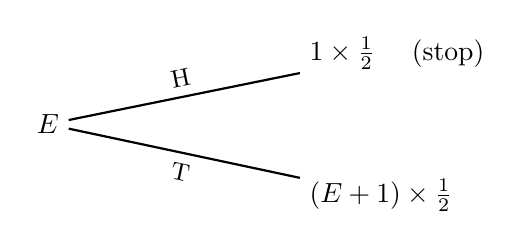
\begin{tikzpicture}[tr]
  \node (e0) at (0,0) {$E$};
  \node[anchor=west] (h) at (3.2,0.9) {$1\times\tfrac12$ \quad (stop)};
  \node[anchor=west] (t) at (3.2,-0.9) {$(E+1)\times\tfrac12$};
  \draw[br] (e0) -- node[lb]{H} (h);
  \draw[br] (e0) -- node[lb,below]{T} (t);
\end{tikzpicture}
\end{center}

\textbf{Answer:}

\[
E=\frac12(1)+\frac12(E+1)
\]

\[
E=1+\frac12E
\quad\Longrightarrow\quad
\frac12E=1
\]

\[
\boxed{E=2}.
\]

\subsection*{Question 2: Expected Rolls Until the First 6}

\textbf{Question:}
A fair six-sided die is rolled until the first 6 appears. What is the expected number of rolls?

\begin{center}
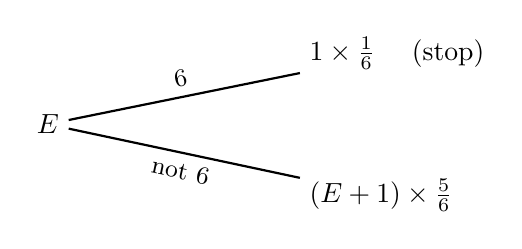
\begin{tikzpicture}[tr]
  \node (e0) at (0,0) {$E$};
  \node[anchor=west] (h) at (3.2,0.9) {$1\times\tfrac16$ \quad (stop)};
  \node[anchor=west] (t) at (3.2,-0.9) {$(E+1)\times\tfrac56$};
  \draw[br] (e0) -- node[lb]{6} (h);
  \draw[br] (e0) -- node[lb,below]{not 6} (t);
\end{tikzpicture}
\end{center}

\textbf{Answer:}

\[
E=\frac16(1)+\frac56(E+1)
\]

\[
E=1+\frac56E
\quad\Longrightarrow\quad
\frac16E=1
\]

\[
\boxed{E=6}.
\]

\subsection*{Question 3: Expected Tosses Until HHT Appears}

\textbf{Question:}
A fair coin is tossed until the pattern HHT first appears. Find the expected number of tosses.

States: $E_0$ = nothing matched, $E_1$ = last toss H, $E_2$ = last two tosses HH.

\begin{center}
\begin{tikzpicture}[tr]
  \node (e0) at (0,0) {$E_0$};
  \node (e1) at (3.2,1.4) {$E_1$};
  \node[anchor=west] (t0) at (3.2,-1.4) {$(E_0+1)\times\tfrac12$};
  \node (e2) at (6.4,2.6) {$E_2$};
  \node[anchor=west] (t1) at (6.4,0.3) {$(E_0+1)\times\tfrac12$};
  \node[anchor=west] (t2) at (9.4,1.5) {$1\times\tfrac12$ \quad (stop)};
  \node[anchor=west] (h2) at (9.4,3.7) {$(E_2+1)\times\tfrac12$};
  \draw[br] (e0) -- node[lb]{H} (e1);
  \draw[br] (e0) -- node[lb,below]{T} (t0);
  \draw[br] (e1) -- node[lb]{H} (e2);
  \draw[br] (e1) -- node[lb,below]{T} (t1);
  \draw[br] (e2) -- node[lb,below]{T} (t2);
  \draw[br] (e2) -- node[lb]{H} (h2);
\end{tikzpicture}
\end{center}

Note that from $E_2$ another H leaves you in $E_2$, since the last two tosses are still HH.

\textbf{Answer:}

Reading the leaves:

\[
E_2=\tfrac12(1)+\tfrac12(E_2+1)\quad\Rightarrow\quad E_2=2,
\]

\[
E_1=\tfrac12(E_2+1)+\tfrac12(E_0+1)=2+\tfrac12E_0,
\]

\[
E_0=\tfrac12(E_1+1)+\tfrac12(E_0+1)\quad\Rightarrow\quad E_0=E_1+2.
\]

Substituting $E_1$ gives $E_0=4+\tfrac12E_0$, so

\[
\boxed{E_0=8}.
\]

\subsection*{Question 4: Random Walk Intuition}

\textbf{Question:}
What is the main idea behind first-step analysis in random-walk problems?

\textbf{Answer:}

A random walk moves between states. The key observation is:

\begin{quote}
After taking the next step, the process is again in a state whose future behavior can be described by the same expectation equations.
\end{quote}

The general form, with $E=0$ at every stopping state, is:

\[
E(\text{current state}) = \sum P(\text{next state})\bigl[E(\text{next state})+1\bigr].
\]

\subsection*{Question 5: Gambler's Ruin Intuition}

\textbf{Question:}
How does first-step analysis help in Gambler's Ruin problems?

\begin{center}
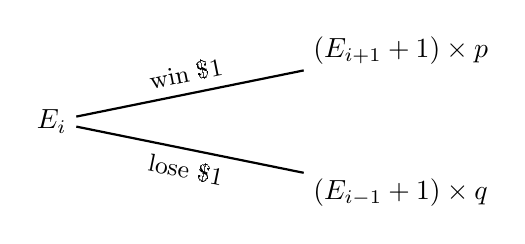
\begin{tikzpicture}[tr]
  \node (ei) at (0,0) {$E_i$};
  \node[anchor=west] (up) at (3.2,0.9) {$(E_{i+1}+1)\times p$};
  \node[anchor=west] (dn) at (3.2,-0.9) {$(E_{i-1}+1)\times q$};
  \draw[br] (ei) -- node[lb]{win \$1} (up);
  \draw[br] (ei) -- node[lb,below]{lose \$1} (dn);
\end{tikzpicture}
\end{center}

\textbf{Answer:}

Suppose a gambler currently has $i$ dollars. If $E_i$ denotes the expected time until ruin or victory from state $i$, then reading the leaves,

\[
E_i=p\,(E_{i+1}+1)+q\,(E_{i-1}+1)=1+pE_{i+1}+qE_{i-1},
\qquad E_0=E_N=0.
\]

\subsection*{Key Takeaway}

\[
\boxed{
E(\text{state})
=
\sum P(\text{branch})\bigl[E(\text{new state})+1\bigr]
}
\]

Draw the tree, write each leaf as (new expectation $+1$) $\times$ probability, and add the leaves.

\end{document}